\chapter{Algorithm for computing Nash Equilibria of Queueing games}

In this section, first we introduce and analyse the \textit{best-response algorithm} as stated in Section 3 of \cite{laan}.

In this section, we consider the problem of transforming a given model of a queueing network game into that of a traditional payoff matrix to be used for finding the Nash Equilibria, if any. As described in Chapter \ref{chap2}, the model consists of a set of $N$ players and $C$ nodes and each player have $\lambda_j$ as the arrival rate of their customers, while each node has service rate $\mu_i$. $R^(j)$ are the sets of routes available to each player.

Here, we consider a discrete and finite strategy space for the players, so the payoffs to be computed will be that of \textit{pure-strategy profiles}, where each cell of the payoff matrix will represent a distinct route chosen by each player.

When the above data is given as input, our algorithm outputs the payoff matrix in which each cell of the matrix gives the payoffs, which are the \textit{Mean sojourn times} of the customers, of each player when following the route that the cell corresponds to. To find the Nash Equilibria, we can assign the goal for each player to be to minimize the mean sojourn time for their customers.



\section{The Algorithm}

The following python code returns the payoff matrix for N-player queueing games with C nodes in the queueing network, with a pure-strategy profile

\lstset{language=Python}
\lstset{frame=lines}
\lstset{caption={Payoff Matrix}}
\lstset{label={lst:code_direct}}
\lstset{basicstyle=\footnotesize}
\begin{lstlisting}
import numpy as np
from itertools import product

def read_floats():
    inp = input()
    inp = list(map(float,filter(lambda x: x!='', inp.split(' '))))
    if len(inp) == 1:
        return inp[0]
    else:
        return tuple(inp)

N, C = map(int, read_floats())
service_rate = read_floats()
arrv_rate = [0]*N
routes = [[] for i in range(N)]

for j in range(N):
    num_routes, arr = read_floats()
    num_routes = int(num_routes)
    arrv_rate[j] = arr
    for _ in range(num_routes):
        #convert to 0 indexed int and remove the first element
        route = list(map(lambda x: int(x)-1, read_floats()))[1:] 
        routes[j].append(route)


idx = 0
def calc_payoffs(S):
    global idx
    idx += 1
    freq_node = [0]*C
    for j in range(N):
        for i in range(len(routes[j])):
            for node in routes[j][i]:
                freq_node[node] += S[j][i]*arrv_rate[j]
    sojourn_node = [0]*C
    for i in range(C):
        assert(service_rate[i] > freq_node[i])
        sojourn_node[i] = 1/(service_rate[i] - freq_node[i])
    expected_waiting_time = [0]*N
    for j in range(N):
        for i in range(len(routes[j])):
            route_wait = 0
            for node in routes[j][i]:
                route_wait += sojourn_node[node]
            expected_waiting_time[j] += route_wait*S[j][i]
    return expected_waiting_time


payoff = np.zeros(tuple(list(len(routes[j]) for j in range(N)) + [N]))
indices = product(*tuple(range(len(routes[j])) for j in range(N)))
for index in indices:
    # index = (1,4,2,0,...) -> corresponding to choices of route
    S = [[0]*len(routes[j]) for j in range(N)]
    for j, choice in enumerate(index):
        S[j][choice] = 1
    payoff[index] = calc_payoffs(S)
print(payoff)
\end{lstlisting}

\subsection{Input format}
The code takes input as follows:\\
The first line contains two numbers: the number of players $N$ and number of nodes $C$.\\
The next line contains $C$ integers denoting the service rates of nodes.\\
Then for each player, the first line contains: number of routes $|R^{(j)}|$ and arrival rate $\lambda^{(j)}$.\\
Then then next $|R^{(j)}|$ lines contains: an integer $k$ followed by $k$ integers $r_1 ~ , ~ r_2 ~ \ldots, ~ r_k$ which denotes a route
$(r_1 ~ , ~ \ldots ~ , ~ r_k)$

\subsection{Output format}
The output is an $|R^{(1)}| \times |R^{(2)}| \times ... \times |R^{(N)}|$ matrix, where each cell is a tuple of size $N$, of Real numbers denoting the \textit{mean sojourn time}.
\begin{remark}
The cell $(i_1 ~ , ~ i_2, ~ \ldots , ~ i_n)$ gives the \textit{payoffs/mean sojourn times} for the action profile $(r_{i_1}^{(1)} ~ , ~ r_{i_2}^{(2)} ~ \ldots , ~ r_{i_N}^{(N)})$. The $j^th$ value in the tuple gives the \textit{mean sojourn time} for player $j$.
\end{remark}


\subsection{Examples}
\begin{example}
\textit{Input:} \\
\begin{verbatim}
2 4 
5 7 6 9 
3 2 
1 2 
2 1 4 
3 2 3 4 
2 2 
1 1 
1 3 
\end{verbatim}
% 2 4 \\
% 5 7 6 9 \\
% 3 2 \\
% 1 2 \\
% 2 1 4 \\
% 3 2 3 4 \\
% 2 2 \\
% 1 1 \\
% 1 3 \\


This is a 2 player game with 4 nodes and the routes for each player are defined in the input in further lines.
The following figure represents the network of queues and the possible routes for the players. \\



\begin{figure}[!htbp]
\label{fig:2P3N_example}
% \centering
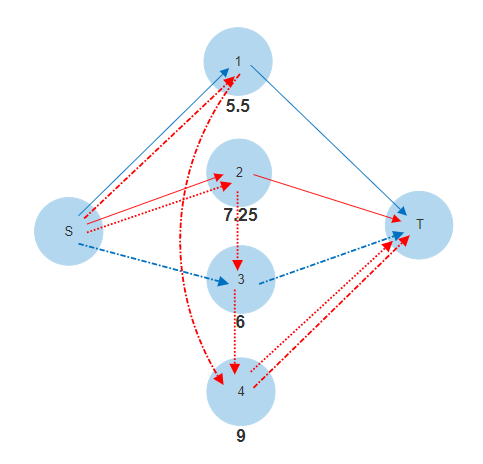
\includegraphics[height=7.5cm]{Example1.png}
\caption{Two-player queueing game with four nodes}
\end{figure}


The red arrows correspond to player 1 and blue correspond to player 2. For multiple paths of the same player, arrows with a different dash pattern are used.

The result from this input is a 2 dimensional payoff-matrix with each cell being a tuple of 2 values, the \textit{mean sojourn time} for each player.

\noindent
\textit{Output:} \\

\begin{table}[!htbp]
    \centering
    \begin{tabular}{cc}
    (0.19047619, 0.28571429) & (0.19047619, 0.25) \\
    (0.80952381, 0.66666667) & (0.42857143, 0.25) \\
    (0.58333333, 0.28571429) & (0.83333333, 0.5)
    \end{tabular}
    \caption{Example 1 - Payoff matrix}
    \label{tab:prog_output1}
\end{table}
% $
% \begin{bmatrix}
% \end{bmatrix}
% $ \\

\vspace{5mm}

This is a $3 \times 2$ matrix, with each row in the $j^{th}$ dimension corresponding to a distinct route for player $j$.
\end{example}

\begin{example}
\textit{Input:}
\begin{verbatim}
3 6
6 6 4.95 4.95 6 6
2 1
3 1 2 3
3 4 5 6
2 2
3 1 2 4
3 3 5 6
2 1
6 1 2 3 4 5 6
1 1
\end{verbatim}
% 3 6 \\
% 6 6 4.95 4.95 6 6 \\
% 2 1 \\
% 3 1 2 3 \\
% 3 4 5 6 \\
% 2 2 \\
% 3 1 2 4 \\
% 3 3 5 6 \\
% 2 1 \\
% 6 1 2 3 4 5 6 \\
% 1 1 \\

So this is a 3 player game with 6 nodes.

The following figure represents the network of queues and the possible routes for the players. \\

\begin{figure}[!htbp]
% \centering
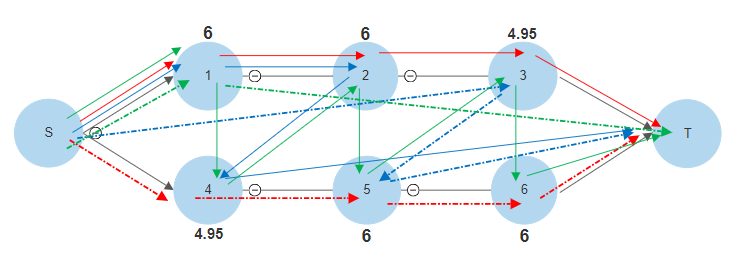
\includegraphics[height=4.5cm]{Example2.png}
\caption{Three-player queueing game with six nodes}
\end{figure}



The red arrows correspond to player 1, blue correspond to player 2 and green correspond to player 3. For multiple paths of the same player, arrows with a different dash pattern are used.

The result from this input is a 3 dimensional payoff-matrix with each cell being a tuple of 3 values, the \textit{mean sojourn time} for each player.

\textit{Output:}
\begin{table}[!htbp]
    \begin{tabular}{|cc|}
    (1.34, 1.51, 2.25) & (1.09, 1.17, 0.50) \\
    (1.55, 1.72, 2.47) & (0.96, 1.01, 0.25)
    \end{tabular}
    % \newline
    % \vspace*{0.8 cm}
    % \newline
    \qquad
    \begin{tabular}{|cc|}
    (1.55, 1.72, 2.47) & (0.91, 1.10, 0.33) \\
    (1.34, 1.51, 2.25) & (0.92 1.01, 0.20)
    \end{tabular}    
    
    
    \caption{Example 2 - Payoff matrix}
    \label{tab:prog_output1}
\end{table}

% $
% \begin{bmatrix}
% (1.33898305, 1.51282051, 2.25180356) & (1.08649789, 1.17231638, 0.5) \\
% (1.55263158, 1.71929825, 2.4724628) & (0.96282051, 1.01282051, 0.25)
% \end{bmatrix}
% $ \\
% $
% \begin{bmatrix}
% (1.55263158, 1.71929825, 2.4724628) & (0.91282051, 1.09615385, 0.333) \\
% (1.33898305, 1.51282051, 2.25180356) & (0.91983122 1.00564972, 0.2)
% \end{bmatrix} 
% $ \\

\vspace{5mm}

This is a $2 \times 2 \times 2$ matrix, with each row in the $j^{th}$ dimension corresponding to a distinct route for player $j$.
\end{example}




% \section{Section-2 Name}
% \begin{definition}\label{abc6}
% Some definition....
% \end{definition}

% \begin{remark}
% Some remark.......
% \end{remark}

% \subsection{Subsection name}

% \begin{theorem}
% Some theorem.......
% \end{theorem}

% \begin{proof}
% Proof is as follows....
% \end{proof}
